% This file was created by matlab2tikz.
%
%The latest updates can be retrieved from
%  http://www.mathworks.com/matlabcentral/fileexchange/22022-matlab2tikz-matlab2tikz
%where you can also make suggestions and rate matlab2tikz.
%
\definecolor{mycolor1}{rgb}{0.00000,0.44700,0.74100}%
\definecolor{mycolor2}{rgb}{0.85000,0.32500,0.09800}%
\definecolor{mycolor3}{rgb}{0.46600,0.67400,0.18800}%
\definecolor{mycolor4}{rgb}{0.49400,0.18400,0.55600}%
%
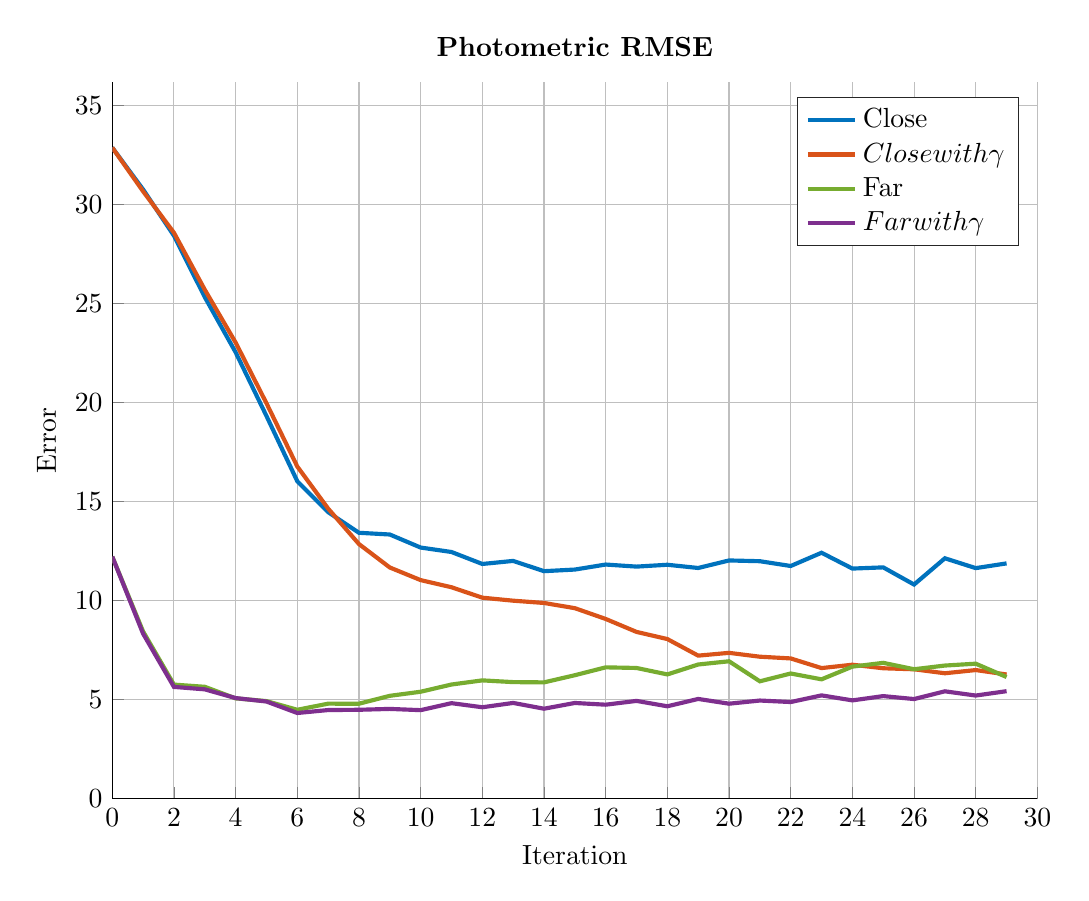
\begin{tikzpicture}

\begin{axis}[%
width=0.969\linewidth,
height=0.75\linewidth,
at={(0\linewidth,0\linewidth)},
scale only axis,
xmin=0,
xmax=30,
xlabel={Iteration},
xmajorgrids,
ymin=0,
ylabel={Error},
ymajorgrids,
axis background/.style={fill=white},
title style={font=\bfseries},
title={Photometric RMSE},
axis x line*=bottom,
axis y line*=left,
legend style={legend cell align=left,align=left,draw=white!15!black}
]
\addplot [color=mycolor1,solid,line width=1.5pt]
  table[row sep=crcr]{%
0	32.8765\\
1	30.7613\\
2	28.4269\\
3	25.3259\\
4	22.539\\
5	19.3246\\
6	16.0249\\
7	14.4648\\
8	13.4227\\
9	13.3361\\
10	12.6765\\
11	12.4527\\
12	11.8476\\
13	12.0018\\
14	11.4839\\
15	11.5655\\
16	11.819\\
17	11.7148\\
18	11.8078\\
19	11.6447\\
20	12.0251\\
21	11.9872\\
22	11.7451\\
23	12.415\\
24	11.6159\\
25	11.6755\\
26	10.809\\
27	12.1347\\
28	11.6383\\
29	11.8771\\
};
\addlegendentry{Close};

\addplot [color=mycolor2,solid,line width=1.5pt]
  table[row sep=crcr]{%
0	32.8765\\
1	30.6668\\
2	28.5774\\
3	25.6998\\
4	23.0307\\
5	19.9675\\
6	16.7695\\
7	14.6451\\
8	12.8529\\
9	11.67\\
10	11.0326\\
11	10.672\\
12	10.1455\\
13	9.99341\\
14	9.87842\\
15	9.6155\\
16	9.07102\\
17	8.41648\\
18	8.0555\\
19	7.21861\\
20	7.35917\\
21	7.16422\\
22	7.0774\\
23	6.58987\\
24	6.75989\\
25	6.5806\\
26	6.52855\\
27	6.32808\\
28	6.49009\\
29	6.26694\\
};
\addlegendentry{$\text{Close with }\gamma$};

\addplot [color=mycolor3,solid,line width=1.5pt]
  table[row sep=crcr]{%
0	12.219\\
1	8.43807\\
2	5.75557\\
3	5.64414\\
4	5.06052\\
5	4.92199\\
6	4.48379\\
7	4.79279\\
8	4.79033\\
9	5.18879\\
10	5.39492\\
11	5.75986\\
12	5.96856\\
13	5.88106\\
14	5.86797\\
15	6.229\\
16	6.6267\\
17	6.59556\\
18	6.26931\\
19	6.77066\\
20	6.93361\\
21	5.9215\\
22	6.31606\\
23	6.02172\\
24	6.66415\\
25	6.85459\\
26	6.53181\\
27	6.71777\\
28	6.81212\\
29	6.13852\\
};
\addlegendentry{Far};

\addplot [color=mycolor4,solid,line width=1.5pt]
  table[row sep=crcr]{%
0	12.219\\
1	8.32782\\
2	5.63938\\
3	5.51586\\
4	5.07539\\
5	4.90134\\
6	4.32102\\
7	4.47033\\
8	4.48355\\
9	4.52778\\
10	4.46472\\
11	4.81814\\
12	4.61121\\
13	4.8298\\
14	4.53792\\
15	4.82781\\
16	4.74083\\
17	4.9326\\
18	4.66009\\
19	5.03098\\
20	4.79117\\
21	4.95051\\
22	4.87511\\
23	5.21122\\
24	4.95826\\
25	5.17446\\
26	5.02563\\
27	5.41652\\
28	5.20287\\
29	5.42374\\
};
\addlegendentry{$\text{Far with }\gamma$};

\addplot [color=mycolor1,dashed,line width=1.5pt,forget plot]
  table[row sep=crcr]{%
0	-1\\
1	-1\\
2	-1\\
3	-1\\
4	-1\\
5	-1\\
6	-1\\
7	-1\\
8	-1\\
9	-1\\
10	-1\\
11	-1\\
12	-1\\
13	-1\\
14	-1\\
15	-1\\
16	-1\\
17	-1\\
18	-1\\
19	-1\\
20	-1\\
21	-1\\
22	-1\\
23	-1\\
24	-1\\
25	-1\\
26	-1\\
27	-1\\
28	-1\\
29	-1\\
};
\addplot [color=mycolor2,dashed,line width=1.5pt,forget plot]
  table[row sep=crcr]{%
0	-1\\
1	-1\\
2	-1\\
3	-1\\
4	-1\\
5	-1\\
6	-1\\
7	-1\\
8	-1\\
9	-1\\
10	-1\\
11	-1\\
12	-1\\
13	-1\\
14	-1\\
15	-1\\
16	-1\\
17	-1\\
18	-1\\
19	-1\\
20	-1\\
21	-1\\
22	-1\\
23	-1\\
24	-1\\
25	-1\\
26	-1\\
27	-1\\
28	-1\\
29	-1\\
};
\addplot [color=mycolor3,dashed,line width=1.5pt,forget plot]
  table[row sep=crcr]{%
0	-1\\
1	-1\\
2	-1\\
3	-1\\
4	-1\\
5	-1\\
6	-1\\
7	-1\\
8	-1\\
9	-1\\
10	-1\\
11	-1\\
12	-1\\
13	-1\\
14	-1\\
15	-1\\
16	-1\\
17	-1\\
18	-1\\
19	-1\\
20	-1\\
21	-1\\
22	-1\\
23	-1\\
24	-1\\
25	-1\\
26	-1\\
27	-1\\
28	-1\\
29	-1\\
};
\addplot [color=mycolor4,dashed,line width=1.5pt,forget plot]
  table[row sep=crcr]{%
0	-1\\
1	-1\\
2	-1\\
3	-1\\
4	-1\\
5	-1\\
6	-1\\
7	-1\\
8	-1\\
9	-1\\
10	-1\\
11	-1\\
12	-1\\
13	-1\\
14	-1\\
15	-1\\
16	-1\\
17	-1\\
18	-1\\
19	-1\\
20	-1\\
21	-1\\
22	-1\\
23	-1\\
24	-1\\
25	-1\\
26	-1\\
27	-1\\
28	-1\\
29	-1\\
};
\end{axis}
\end{tikzpicture}%